\documentclass[11pt,reqno]{amsart}
\usepackage[margin=1.15in]{geometry}
\usepackage{amsmath,amssymb,amsthm,mathtools}
\usepackage{graphicx}
\usepackage{booktabs}
\usepackage[colorlinks=true,linkcolor=blue,citecolor=blue,urlcolor=blue]{hyperref}
\usepackage{microtype}

\theoremstyle{plain}
\newtheorem{theorem}{Theorem}
\newtheorem{proposition}[theorem]{Proposition}
\newtheorem{corollary}[theorem]{Corollary}
\newtheorem{lemma}[theorem]{Lemma}
\newtheorem{conjecture}[theorem]{Conjecture}
\theoremstyle{definition}
\newtheorem{definition}[theorem]{Definition}
\newtheorem{remark}[theorem]{Remark}
\newtheorem{observation}[theorem]{Observation}

\DeclareMathOperator{\sqf}{sqf}
\newcommand{\Art}{\mathrm{A}}
\newcommand{\Z}{\mathbb{Z}}
\newcommand{\Q}{\mathbb{Q}}

\begin{document}

\title[The sign of the consecutive-prime Artin correlation]
{The sign of the consecutive-prime Artin correlation}

\author{Josh Bald}
\address{Ontario, Canada}
\email{jpbald93@gmail.com}

\subjclass[2020]{Primary 11A07; Secondary 11N05, 11N13, 11Y16, 11Y60}
\keywords{Artin's conjecture, primitive roots, consecutive primes,
quadratic characters, Lemke Oliver--Soundararajan bias}

\date{\today}

\begin{abstract}
For a non-square base $a$, earlier papers in this series measured the
correlation $\delta(a)$ between the primitive-root (``Artin'') statuses of
consecutive primes and found it negative for every base examined, with a
single positive exception at $a = 15$. Here we settle the qualitative
question of which sign $\delta$ takes and why, by measuring $\delta(a)$ for
all $64$ non-square bases $a \le 105$ with squarefree part exceeding $1$,
over the $50{,}847{,}531$ consecutive prime pairs below $10^9$. Sixteen bases
have $\delta(a) > 0$, fifteen of them at $|z| > 5$; positivity is not an
anomaly of $a=15$ but a regime. The sixteen positive bases are exactly the
sixteen bases of largest conductor-adjusted class imbalance: every positive
base has conductor $f \ge 60$, every base with $f \le 44$ is negative, and
the sign is organised by a \emph{class-competition} decomposition of
$\delta$ into a between-class term (gap classes with forced equal or opposite
quadratic-residue status compete) and a within-class term (the Lemke
Oliver--Soundararajan repulsion acts inside each class). The between-class
term is negative for $62$ of $64$ bases; the within-class term is what
changes sign, and a character-level statistic $T(a)$, computable from the
conductor alone in a few milliseconds without any prime data, satisfies:
$T(a) > 0$ for all $16$ positive bases, and every base with $T(a) \le 0$ is
negative. A calibrated one-parameter model reaches $R^2 = 0.958$ against the
measured $\delta$ over all $64$ bases and predicts the correct sign for
$60$. Finally we track the positive exemplar $a = 15$ to $10^{10}$
($455{,}052{,}508$ pairs): the sign persists decisively
($\delta = +0.00465$, $z = 99$), but the magnitude decays \emph{faster} than
the $1/\log x$ rate suggested previously --- refuting the conjecture, made in
the fourth paper of this series, that $\delta(15;x)$ grows more positive
with $x$.
\end{abstract}

\maketitle

\section{Introduction}
\label{sec:intro}

Call a prime $p$ an \emph{Artin prime base $a$} if $a$ is a primitive root
modulo $p$. For consecutive primes $p_n < p_{n+1} \le x$ define
\begin{equation}
\label{eq:delta}
  \delta(a; x) \;=\; P\bigl(p_{n+1} \in \Art_a \mid p_n \in \Art_a\bigr)
             \;-\; P\bigl(p_{n+1} \in \Art_a \mid p_n \notin \Art_a\bigr),
\end{equation}
probabilities being proportions over the consecutive pairs below $x$. The
first paper in this series measured $\delta(10;10^9) = -0.01414$
($z \approx -101$); the second extended the measurement to eleven bases, all
negative, and proved unconditional \emph{exclusion laws}: explicit gap
classes modulo the conductor $f$ of the quadratic character
$\chi_a$ in which no consecutive pair can be doubly Artin. A fourth paper,
measuring the mixed two-base statistic, encountered the first positive case,
$\delta(15;10^9) = +0.0122$ ($z = 87$) --- a base for which consecutive
primes \emph{attract} in Artin status.

A single positive base among a dozen looks like an anomaly. This paper
asks the natural question: \emph{what determines the sign of $\delta(a)$?}
We answer it in three steps.

\begin{enumerate}
\item \textbf{A census} (Section~\ref{sec:census}). We measure $\delta(a;10^9)$
      for all $64$ non-square bases $2 \le a \le 105$ with $\sqf(a) > 1$,
      over all $50{,}847{,}531$ consecutive prime pairs below $10^9$.
      Sixteen bases are positive --- positivity is a regime, not an outlier
      --- and the positive and negative bases separate cleanly by conductor:
      every positive base has $f \ge 60$, and every base with $f \le 44$ is
      negative.
\item \textbf{A mechanism} (Section~\ref{sec:competition}). We decompose
      $\delta$ into a \emph{between-class} term --- driven by the gap classes
      mod $f$ in which quadratic-residue status is forced equal or opposite,
      the mechanism of the exclusion laws --- and a \emph{within-class} term,
      driven by the Lemke Oliver--Soundararajan bias
      \cite{LOS2016} acting inside each class. The between-class term
      is negative for $62$ of the $64$ bases. The within-class term is what
      changes sign, and it does so according to a character-level statistic
      $T(a)$ computable from $\chi_a$ alone --- no prime data required.
      $T(a) > 0$ holds for all sixteen positive bases, and no base with
      $T(a) \le 0$ is positive.
\item \textbf{A stress test} (Section~\ref{sec:decay}). We push the positive
      exemplar $a = 15$ to $x = 10^{10}$. The sign survives decisively
      ($z = 99$), but the magnitude drops from $+0.0122$ to $+0.00465$ ---
      a factor $2.6$, where the $1/\log x$ decay of the underlying bias
      would predict a factor $1.11$. This \emph{refutes} the conjecture,
      recorded in the fourth paper, that $\delta(15;x)$ should become more
      positive as $x$ grows, and we replace it with a corrected one
      (Conjecture~\ref{conj:decay}).
\end{enumerate}

Throughout, $d = \sqf(a)$ is the squarefree part of $a$, and
$f = f(a)$ the conductor of the quadratic character
$\chi_a = \left(\frac{d}{\cdot}\right)$, i.e.\ $f = |D|$ for $D$ the
discriminant of $\Q(\sqrt{d})$. All counts are exact; standard errors for
$\delta$ are the usual binomial errors for a difference of proportions, and
$z = \delta/\mathrm{se}$.

\section{The census: sixteen positive bases}
\label{sec:census}

We computed Artin status for all $64$ bases simultaneously, factoring each
$p - 1$ once (the computational scheme of the second paper in this series;
the entire run takes under two hours on two cores and writes no intermediate
table). Table~\ref{tab:census} lists all bases with $\delta > 0$ together
with the most negative bases for contrast.

\begin{table}[t]
\centering
\caption{All sixteen positive bases at $x = 10^9$ (top block, sorted by
$\delta$), and the five most negative bases (bottom block). $w_{\mathrm{exc}}$
and $w_{\mathrm{prs}}$ are the fractions of consecutive pairs lying in
exclusion and preserving gap classes respectively; $T$ is the sign statistic
of Section~\ref{sec:competition}.}
\label{tab:census}
\begin{tabular}{rrrrrrr}
\toprule
$a$ & $\sqf(a)$ & $f$ & $\delta(a;10^9)$ & $z$ & $w_{\mathrm{exc}}$ & $T(a)$ \\
\midrule
$30$  & $2\cdot3\cdot5$   & $120$ & $+0.026445$ & $+188.0$ & $0.021$ & $+0.0084$ \\
$15$  & $3\cdot5$         & $60$  & $+0.012196$ & $+86.8$  & $0.094$ & $+0.0022$ \\
$39$  & $3\cdot13$        & $156$ & $+0.011777$ & $+83.9$  & $0.007$ & $+0.0055$ \\
$105$ & $3\cdot5\cdot7$   & $105$ & $+0.011248$ & $+80.1$  & $0.003$ & $+0.0081$ \\
$70$  & $2\cdot5\cdot7$   & $280$ & $+0.010270$ & $+73.1$  & $0.000$ & $+0.0028$ \\
$55$  & $5\cdot11$        & $220$ & $+0.010049$ & $+71.6$  & $0.000$ & $+0.0039$ \\
$42$  & $2\cdot3\cdot7$   & $168$ & $+0.009158$ & $+65.2$  & $0.010$ & $+0.0074$ \\
$66$  & $2\cdot3\cdot11$  & $264$ & $+0.008121$ & $+57.8$  & $0.004$ & $+0.0031$ \\
$51$  & $3\cdot17$        & $204$ & $+0.006473$ & $+46.1$  & $0.005$ & $+0.0042$ \\
$35$  & $5\cdot7$         & $140$ & $+0.004542$ & $+32.4$  & $0.021$ & $+0.0056$ \\
$87$  & $3\cdot29$        & $348$ & $+0.003585$ & $+25.6$  & $0.002$ & $+0.0015$ \\
$95$  & $5\cdot19$        & $380$ & $+0.003417$ & $+24.4$  & $0.001$ & $+0.0016$ \\
$26$  & $2\cdot13$        & $104$ & $+0.001614$ & $+11.5$  & $0.008$ & $+0.0005$ \\
$78$  & $2\cdot3\cdot13$  & $312$ & $+0.000924$ & $+6.6$   & $0.003$ & $+0.0022$ \\
$38$  & $2\cdot19$        & $152$ & $+0.000731$ & $+5.2$   & $0.005$ & $+0.0009$ \\
$102$ & $2\cdot3\cdot17$  & $408$ & $+0.000425$ & $+3.0$   & $0.002$ & $+0.0011$ \\
\midrule
$17$  & $17$ & $17$ & $-0.033025$ & $-236.7$ & $0$      & $-0.0123$ \\
$21$  & $3\cdot7$ & $21$ & $-0.038345$ & $-275.2$ & $0.053$ & $-0.0123$ \\
$13$  & $13$ & $13$ & $-0.042573$ & $-305.6$ & $0$      & $-0.0148$ \\
$3$   & $3$  & $12$ & $-0.046676$ & $-335.4$ & $0.531$  & $-0.0156$ \\
$2$   & $2$  & $8$  & $-0.050199$ & $-361.0$ & $0.264$  & $-0.0196$ \\
\bottomrule
\end{tabular}
\end{table}

Three empirical regularities stand out.

\begin{observation}[Conductor threshold]
\label{obs:threshold}
Every positive base has $f \ge 60$; every base with $f \le 44$ is negative.
The two regimes overlap in $60 \le f \le 412$: large conductor is necessary
but not sufficient for positivity.
\end{observation}

\begin{observation}[Composite squarefree part]
\label{obs:composite}
Every positive base has composite squarefree part. No prime $d$ gives a
positive $\delta$ in our range; the positive bases are exactly products of
two or three distinct primes (with or without the factor $2$).
\end{observation}

\begin{observation}[Magnitude ordering]
\label{obs:ordering}
Among negative bases, $|\delta|$ decreases with $f$ (the conductor law of the
second paper, $r(\log f, |\delta|) = -0.96$ over its eleven bases, persists
over $48$ negative bases here). The positive $\delta$ are all small
($\max \delta = +0.0264$, versus $\min \delta = -0.0666$): positivity is a
weak-signal regime.
\end{observation}

Fifteen of the sixteen positive bases exceed $z = 5$; positivity is not a
fluctuation. (The marginal case $a = 102$, $z = 3.0$, we count as positive
but unconfirmed.)

\section{Class competition: where the sign comes from}
\label{sec:competition}

\subsection{The decomposition}
Fix a base $a$ with conductor $f$. Each consecutive pair $(p_n, p_{n+1})$
falls in a \emph{gap class} $g \equiv p_{n+1} - p_n \pmod f$. Within a class,
the pair $(\chi_a(p_n), \chi_a(p_{n+1}))$ of quadratic-character values is
constrained --- in an \emph{exclusion} class (second paper's terminology) the
values are forced opposite, so the pair can never be doubly Artin; in a
\emph{preserving} class they are forced equal, which \emph{favours} double-Artin
pairs; in the remaining (\emph{mixed}) classes both possibilities occur.

Write $\delta = \delta_{\mathrm{between}} + \delta_{\mathrm{within}}$, where
$\delta_{\mathrm{between}}$ is the value $\delta$ would take if, within each
gap class, Artin statuses were independent with the class-conditional
marginal frequencies (so all dependence comes from \emph{which} class the
pair falls in and the class-level character constraints), and
$\delta_{\mathrm{within}} = \delta - \delta_{\mathrm{between}}$ collects the
dependence surviving inside classes. Both terms are computed exactly from
the per-class $2\times2$ contingency tables.

\begin{observation}
\label{obs:between}
$\delta_{\mathrm{between}} < 0$ for $62$ of the $64$ bases (the exceptions,
$a = 5$ and $a = 21$, have the two smallest conductors among bases with
exclusion classes). Class competition is a systematically negative force:
exclusion classes forbid double-Artin pairs outright, and even for mixed
classes the character constraints anticorrelate.
\end{observation}

\begin{observation}
\label{obs:within}
$\delta_{\mathrm{within}} > 0$ for $49$ of the $64$ bases --- including
\emph{all} sixteen positive ones and thirty-three negative ones. The
within-class term is the positive force, and the observed sign of
$\delta(a)$ is the outcome of the competition between the two.
\end{observation}

At small conductor the between-class term is large (few classes, heavy
character constraints per class: e.g.\ base $3$ has half of all pairs in
exclusion classes) and dominates: $\delta < 0$. At large conductor the
constrained classes carry a tiny fraction of pairs
($w_{\mathrm{exc}} \le 2\%$ for most positive bases,
Table~\ref{tab:census}), the between term shrinks toward a common floor
$\approx -0.013$, and the within-class term can win.

\subsection{Why the within-class term can be positive}
The within-class positivity has a concrete source in the Lemke
Oliver--Soundararajan bias \cite{LOS2016}. Being Artin base $a$ requires, first
of all, $\chi_a(p) = -1$: the prime must lie in one of the $\varphi(f)/2$
non-residue classes mod $f$. The LOS bias makes a prime \emph{reluctant} to
repeat its own residue class; for a prime in a non-residue class, the
repelled class is one of the ``Artin-eligible'' ones, and the displaced
probability spreads over \emph{all} other classes --- of which, at large $f$,
half are again non-residue classes. The net within-class effect on the
\emph{binary} variable $\chi = -1$ is then a second-order competition: the
self-repulsion removes weight from one eligible class, while the surplus
lands on eligible and ineligible classes in nearly equal measure. Whether
the eligible side gains or loses depends on the character-weighted average
of the LOS transition matrix over the classes of each sign --- a quantity
determined by $\chi_a$ alone.

This motivates the following statistic. For each even shift $g$ modulo $f$
let $c(g)$ be the fraction, over admissible residues $r$ mod $f$ (both $r$
and $r+g$ coprime to $f$), with $\chi_a(r) = \chi_a(r+g) = -1$; let $w_g$ be
the measured fraction of consecutive pairs in class $g$; and set
\begin{equation}
\label{eq:T}
  T(a) \;=\; \sum_{g} w_g\, c(g) \;-\; \tfrac14 .
\end{equation}
Under class-level independence with equidistributed character values,
$c(g) = 1/4$ identically and $T = 0$; positive $T$ means the gap-class
mixture, weighted by where consecutive pairs actually fall, over-supplies
classes in which both primes can be non-residues simultaneously.

\begin{observation}[Sign criterion]
\label{obs:sign}
Over all $64$ bases: $T(a) > 0$ for every one of the $16$ positive bases,
and every base with $T(a) \le 0$ has $\delta(a) < 0$. Thus $T > 0$ is
necessary for positivity. It is not sufficient: $21$ negative bases have
$T > 0$, but they are precisely the weak-signal bases --- all have
$|\delta| \le 0.0104$, and $16$ of the $21$ have $|\delta| \le 0.0027$,
against positive-side magnitudes up to $+0.0264$.
\end{observation}

Calibrating a single slope on the model value
$\delta_{\mathrm{model}}(a) \propto T(a)$ (ordinary least squares over the
$64$ bases) gives
\[
  \delta \approx 1.053\,\delta_{\mathrm{model}} - 0.0029,
  \qquad R^2 = 0.958,
  \qquad r\bigl(T, \delta\bigr) = 0.971,
\]
with the correct sign for $60$ of $64$ bases; the four misclassified
($a = 26, 38, 102$ predicted negative but measured weakly positive;
$a = 91$ the reverse) all have $|\delta| < 0.0017$, i.e.\ they sit inside
the intercept's own width. The intercept $-0.0029$ is the within-class LOS
repulsion floor that $T$, a character-combinatorial quantity, does not see.
Figure~\ref{fig:sign} displays the fit.

\begin{figure}[t]
\centering
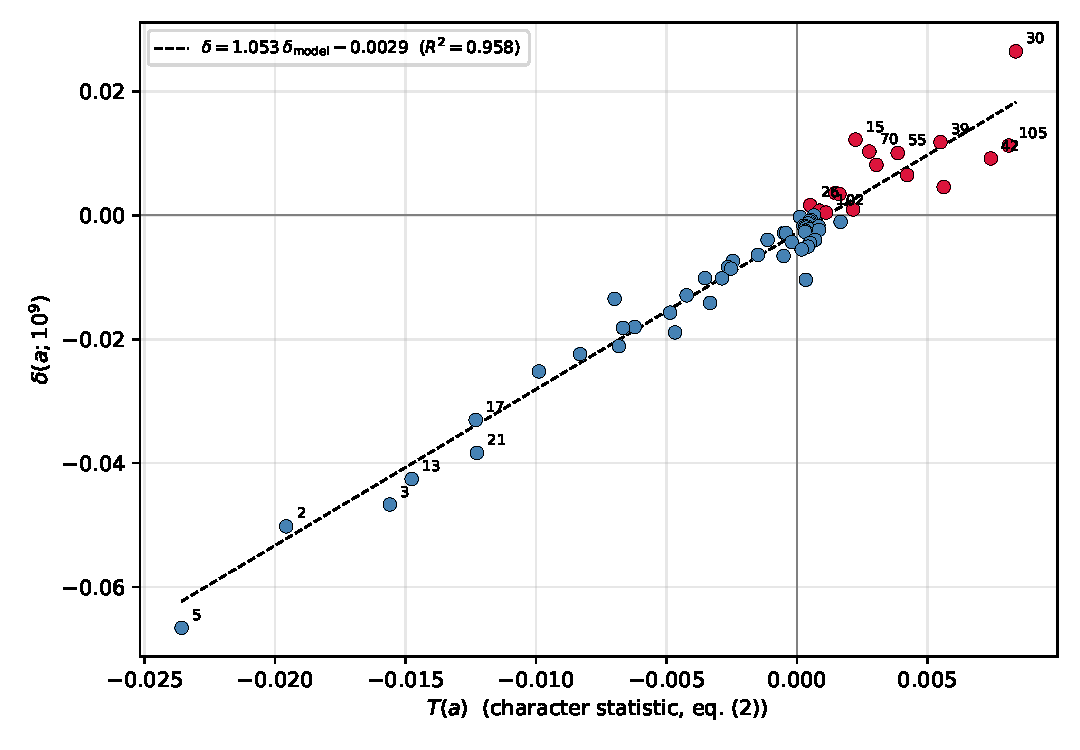
\includegraphics[width=0.72\textwidth]{fig_sign_T.pdf}
\caption{Measured $\delta(a;10^9)$ against the character statistic $T(a)$
for all $64$ bases. Red points: the sixteen positive bases. The dashed line
is the one-parameter calibration $\delta = 1.053\,\delta_{\mathrm{model}} -
0.0029$ ($R^2 = 0.958$). No base with $T \le 0$ is positive.}
\label{fig:sign}
\end{figure}

\begin{remark}
$T(a)$ is computable from the conductor and character table alone ---
milliseconds of computation, no prime data. The sign of the consecutive-prime
Artin correlation for a given base can therefore be predicted before any
sieve is run, up to the weak-signal band $|\delta| \lesssim 0.003$ where the
LOS floor competes with the class mixture.
\end{remark}

\begin{remark}
Observation~\ref{obs:composite} (composite $d$) follows heuristically from
the structure of $T$: for prime $d$ the character $\chi_a$ has a single
prime-discriminant component, the constrained classes are few but heavily
weighted at small $f = d$ or $4d$, and the between-class term dominates. For
composite $d$ the conductor is a product, the constrained classes splinter
into thin slices of the gap distribution, and the class-mixture term
\eqref{eq:T} --- which aggregates over many nearly-independent components ---
can tip positive. We do not prove this; the census verifies it for all
$64$ bases in range.
\end{remark}

\section{The decay of \texorpdfstring{$\delta(15;x)$}{delta(15;x)}: a
conjecture refuted}
\label{sec:decay}

The fourth paper in this series, having found $\delta(15;10^9) = +0.0122$,
conjectured that $\delta(15;x)$ should become \emph{more} positive as $x$
grows: the reasoning was that the within-class LOS repulsion decays like
$1/\log x$ while the class-composition effects do not, so the positive
between/mixture contribution should progressively dominate.

We tested this by extending the computation for $a = 15$ to $x = 10^{10}$:
$455{,}052{,}509$ primes, $455{,}052{,}508$ consecutive pairs, exact counts.
The result:
\[
  \delta(15;10^9) = +0.012196 \;(z = 86.8), \qquad
  \delta(15;10^{10}) = +0.004646 \;(z = 99.0).
\]
The sign persists, at higher significance (nine times the sample). But the
magnitude \emph{fell} by a factor $2.63$ --- and a pure $1/\log x$ decay
across one decade would give a factor of only
$\log 10^{10} / \log 10^{9} = 1.11$. The conjecture is refuted on both
counts: $\delta(15;x)$ is not growing, and its decay is much faster than the
first-order LOS rate.

We record what the data now support:

\begin{conjecture}
\label{conj:decay}
$\delta(15;x) > 0$ for all sufficiently large $x$, and
$\delta(15;x) \to \delta_\infty(15) \ge 0$ as $x \to \infty$. More
generally, for every base $a$, $\delta(a;x)$ tends to a limit
$\delta_\infty(a)$ --- which the companion model paper predicts to be small
but in general \emph{nonzero}, driven by the singular-series dependence of
gap counts on their class mod $f$ --- and the sign of $\delta(a;x)$ for
large $x$ is that of $T(a)$ computed with the limiting gap-class weights,
for every $a$ with $T(a)$ bounded away from $0$.
\end{conjecture}

We deliberately do not conjecture $\delta_\infty(a) = 0$. The companion
paper on the conditional Hardy--Littlewood model derives, under GRH and a
Hardy--Littlewood-type hypothesis, a nonzero limiting value: the
residue-bias (LOS) component of $\delta$ decays like $1/\log x$, but the
gap-class mixture component does not vanish, because the Hardy--Littlewood
singular series makes the limiting weights $w_g$ genuinely non-uniform
across classes mod $f$. On that picture the fast decay observed here is the
transient: $\delta(15;x)$ is falling from an LOS-inflated value toward a
small positive Hardy--Littlewood limit, and a drop by $2.6\times$ over one
decade --- far faster than the $1.11\times$ of a pure $1/\log x$ law --- is
what a difference of two decaying terms of common origin looks like while
the transient dominates. Our two heights cannot separate a small nonzero
limit from a $1/(\log x)^2$ decay to zero; a $10^{11}$--$10^{12}$ run for
this single base would.

\section{Data and computation}
\label{sec:computation}

The $64$-base census reuses the one-pass scheme of the second paper: a
segmented sieve of Eratosthenes enumerates the primes to $10^9$; each
$p - 1$ is factored once by trial division over primes below $10^5$ plus
cofactor; primitive-root status for all $64$ bases is tested by the standard
criterion ($a^{(p-1)/\ell} \not\equiv 1$ for all prime $\ell \mid p-1$) with
$128$-bit modular exponentiation, and $2 \times 2$ contingency counts are
accumulated globally and per gap class. The census takes under two hours on
two cores; the $10^{10}$ single-base run for $a = 15$ takes about nine
hours. The character-level quantities ($f$, class types, $c(g)$, $T$) are
computed independently in exact arithmetic with \texttt{sympy}. Standard
errors are binomial; at $5 \times 10^7$ pairs the resolution is
$|\delta| \approx 6 \times 10^{-4}$ at $z = 4$.

All code, exact contingency tables, and analysis scripts are available in
the public repository cited below.

\section{Discussion}
\label{sec:discussion}

The sign of the consecutive-prime Artin correlation is not mysterious, and
it is not a property of exotic individual bases. It is the visible outcome
of a competition between two forces of common origin: the gap-class
character constraints (always anticorrelating, dominant at small conductor)
and the class-mixture surplus of doubly-eligible residues (positive
precisely when $T(a) > 0$, able to win only when the constrained classes are
thin, i.e.\ at large conductor). Both forces are inherited from the joint
residue distribution of consecutive primes; neither involves any property of
primitive roots beyond the quadratic obstruction. In this sense the sign
question for $\delta(a)$ is a question about quadratic characters of
consecutive primes, resolved by the Lemke Oliver--Soundararajan framework,
with the Artin condition serving as a fixed nonlinear readout.

Three items remain open. First, sufficiency: $T > 0$ is necessary for
positivity in our census but not sufficient, and the residual negative floor
($\approx -0.003$) that $T$ misses should be derivable from the LOS
within-class repulsion --- the companion model paper takes this up. Second,
the decay rate of $\delta(15;x)$, and more generally of any positive-$T$
base, needs a third decade of data. Third, Observation~\ref{obs:composite}
--- no prime squarefree part is positive --- is verified only to $a \le 105$
and deserves either a counterexample at larger prime $d$ (the trend of $T$
with $f = d$ suggests $T$ remains negative for prime $d$, but slowly) or a
proof.

\section*{Acknowledgements}
The author thanks the developers of the open-source tools used in this work
(GCC, Python, \texttt{sympy}, \texttt{matplotlib}).

\subsection*{Use of generative AI}
The author used Anthropic's Claude (models Claude Opus 4.5 and Claude
Opus 5) as an assistant: for drafting and revising exposition, for writing
and debugging the sieve and analysis programs, and for exploratory
discussion of the class-competition mechanism. In the interest of
transparency we record that the refuted conjecture of
Section~\ref{sec:decay} (that $\delta(15;x)$ grows more positive) was
originally proposed during AI-assisted exploration in the fourth paper of
this series, and was tested and refuted here on the evidence. All
mathematical claims in this paper were verified computationally from exact
counts, and the author is solely responsible for the content.

\section*{Declaration of interest}
The author reports there are no competing interests to declare.

\section*{Funding}
This research received no external funding.

\section*{Data availability}
All code and results are publicly available at
\url{https://github.com/jpbald93/consecutive-artin}, including the $64$-base
census program, the $10^{10}$ run for base $15$, the exact contingency
tables underlying Table~\ref{tab:census}, the sign-analysis script computing
$T(a)$ and the class-competition decomposition, and the script reproducing
Figure~\ref{fig:sign}.

\begin{thebibliography}{99}

\bibitem{GarciaKahoroLuca2019}
S.~R. Garcia, E.~Kahoro, and F.~Luca,
\emph{Primitive root bias for twin primes},
Exp. Math. \textbf{28} (2019), no.~2, 151--160.

\bibitem{HardyLittlewood1923}
G.~H. Hardy and J.~E. Littlewood,
\emph{Some problems of `Partitio numerorum'; III: On the expression of a
number as a sum of primes},
Acta Math. \textbf{44} (1923), 1--70.

\bibitem{Hooley1967}
C.~Hooley,
\emph{On Artin's conjecture},
J. Reine Angew. Math. \textbf{225} (1967), 209--220.

\bibitem{Kimmel2024}
S.~Kimmel,
\emph{Consecutive primes and quadratic residues},
Acta Arith. \textbf{216} (2024), 329--348.

\bibitem{KST2025}
O.~Klurman, I.~E. Shparlinski, and J.~Ter\"av\"ainen,
\emph{On the distribution of primitive roots in short intervals},
Bull. Lond. Math. Soc. \textbf{57} (2025), 2429--2443.

\bibitem{LOS2016}
R.~J. Lemke~Oliver and K.~Soundararajan,
\emph{Unexpected biases in the distribution of consecutive primes},
Proc. Natl. Acad. Sci. USA \textbf{113} (2016), no.~31, E4446--E4454.

\bibitem{Lenstra1977}
H.~W. Lenstra, Jr.,
\emph{On Artin's conjecture and Euclid's algorithm in global fields},
Invent. Math. \textbf{42} (1977), 201--224.

\bibitem{Moree2012}
P.~Moree,
\emph{Artin's primitive root conjecture --- a survey},
Integers \textbf{12A} (2012), Article A13, 100~pp.

\bibitem{Pollack2014}
P.~Pollack,
\emph{Bounded gaps between primes with a given primitive root},
Algebra Number Theory \textbf{8} (2014), no.~7, 1769--1786.

\end{thebibliography}

\end{document}
